% ============================================================
% TuitionHub BD — Complete System Design Document
% Compile with: xelatex tuitionhub-bd-design.tex
% ============================================================
\documentclass[12pt,a4paper,twoside]{report}

% ── Packages ──
\usepackage[margin=1in, headheight=14pt]{geometry}
\usepackage{fontspec}
\usepackage{xcolor}
\usepackage{tikz}
\usetikzlibrary{positioning,shapes,arrows,arrows.meta,fit,backgrounds,calc,decorations.pathreplacing,matrix}
\usepackage{booktabs}
\usepackage{longtable}
\usepackage{tabularx}
\usepackage{enumitem}
\usepackage{hyperref}
\usepackage{listings}
\usepackage{caption}
\usepackage{float}
\usepackage{titlesec}
\usepackage{fancyhdr}
\usepackage{graphicx}
\usepackage{wrapfig}
\usepackage[backend=bibtex]{biblatex}
\newcommand{\checkmark}{\ding{51}}
\usepackage{pifont}

% ── Colors ──
\definecolor{primary}{HTML}{1E40AF}
\definecolor{secondary}{HTML}{3B82F6}
\definecolor{accent}{HTML}{06B6D4}
\definecolor{success}{HTML}{10B981}
\definecolor{warning}{HTML}{F59E0B}
\definecolor{danger}{HTML}{EF4444}
\definecolor{dark}{HTML}{1F2937}
\definecolor{light}{HTML}{F3F4F6}
\definecolor{codebg}{HTML}{F8F9FA}
\definecolor{blueprint}{HTML}{DBEAFE}

% ── Hyperlinks ──
\hypersetup{
    colorlinks=true,
    linkcolor=primary,
    urlcolor=secondary,
    citecolor=accent
}

% ── Listings Style ──
\lstdefinestyle{code}{
    backgroundcolor=\color{codebg},
    basicstyle=\footnotesize\ttfamily,
    breaklines=true,
    frame=single,
    rulecolor=\color{gray!30},
    numbers=left,
    numberstyle=\tiny\color{gray},
    keywordstyle=\color{primary}\bfseries,
    commentstyle=\color{green!50!black},
    stringstyle=\color{accent}
}

% ── Section Formatting ──
\titleformat{\chapter}[display]
    {\normalfont\Huge\bfseries\color{primary}}
    {\chaptertitlename\ \thechapter}{20pt}{\Huge}
\titleformat{\section}
    {\normalfont\Large\bfseries\color{primary!80!black}}
    {\thesection}{1em}{}
\titleformat{\subsection}
    {\normalfont\large\bfseries\color{primary!60!black}}
    {\thesubsection}{1em}{}

% ── Header/Footer ──
\pagestyle{fancy}
\fancyhf{}
\fancyhead[LE,RO]{\small\textcolor{primary}{TuitionHub BD --- Design Document}}
\fancyhead[RE,LO]{\small\leftmark}
\fancyfoot[CE,CO]{\thepage}
\renewcommand{\headrulewidth}{0.5pt}

% ── TikZ Styles ──
\tikzset{
    block/.style={rectangle, draw, rounded corners=4pt, minimum width=2.8cm, minimum height=1cm, align=center, font=\small\bfseries, text=white},
    container/.style={rectangle, draw, dashed, rounded corners=6pt, fill=blueprint, inner sep=8pt, font=\small\bfseries\color{primary}},
    arrow/.style={-{Stealth[scale=1.2]}, thick, color=dark!60},
    db/.style={cylinder, draw, shape border rotate=90, minimum width=2cm, minimum height=1cm, aspect=0.25, font=\small\bfseries},
    role/.style={ellipse, draw, minimum width=2.5cm, minimum height=1cm, align=center, font=\small\bfseries},
    note/.style={rectangle, draw, dotted, rounded corners=3pt, fill=yellow!10, font=\small\itshape}
}

% ============================================================
\begin{document}

% ── Title Page ──
\begin{titlepage}
\centering
\vspace*{3cm}

\color{primary}
{\Huge\bfseries TuitionHub BD}\\[0.5cm]
{\LARGE\color{secondary} System Design Document}\\[2cm]

\color{dark}
{\large Version 1.0}\\[0.3cm]
{\large July 2026}\\[2cm]

\rule{0.6\textwidth}{0.5mm}\\[1cm]

{\large\textbf{A Nationwide Tuition Marketplace for Bangladesh}}\\[0.5cm]
{\large Connecting University Students with Families Seeking Tutors}\\[2cm]

\rule{0.6\textwidth}{0.5mm}\\[1cm]

{\small\textit{Prepared for internal architecture review --- Implementation follows TDD methodology}}\\[0.5cm]
{\small\textcolor{gray}{Tech Stack: Next.js 15 + ASP.NET Core 9 + PostgreSQL 16 + FastAPI (AI/ML) + Docker}}

\vfill
\end{titlepage}

% ── Table of Contents ──
\tableofcontents
\clearpage

% ============================================================
\chapter{Executive Summary}
% ============================================================

\section{Purpose}
TuitionHub BD is a multi-sided marketplace platform that connects \textbf{university students seeking tuition jobs (Tutors)} with \textbf{guardians or students looking for qualified private tutors (Guardians)} across Bangladesh. The platform is managed by a \textbf{Super Admin} and supported by \textbf{Sub Admins}.

\section{Core Objectives}
\begin{itemize}
    \item Create a trusted, transparent marketplace for private tuition in Bangladesh
    \item Implement a fair, multi-factor tutor matching system driven by rules and ML, not LLMs
    \item Provide role-specific dashboards for all four user types
    \item Enable secure communication, verified profiles, and reputation-based trust scoring
    \item Build for scale --- millions of users across all divisions of Bangladesh
\end{itemize}

\section{Four Primary Roles}
\begin{center}
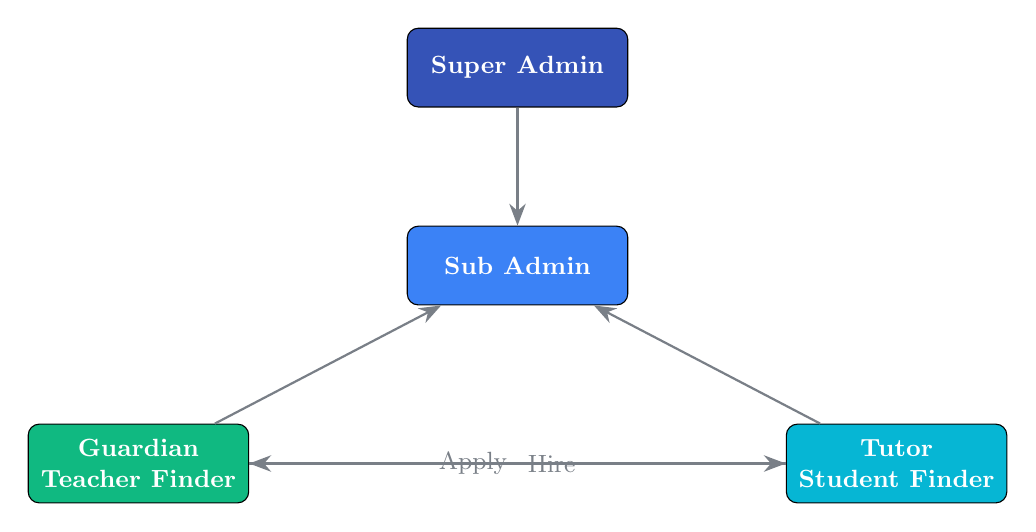
\begin{tikzpicture}[node distance=1.5cm]
    \node[block, fill=primary!90] (super) {Super Admin};
    \node[block, fill=secondary, below=of super] (sub) {Sub Admin};
    \node[block, fill=success, below left=1.5cm and 2cm of sub] (guardian) {Guardian \\ Teacher Finder};
    \node[block, fill=accent, below right=1.5cm and 2cm of sub] (tutor) {Tutor \\ Student Finder};
    \draw[arrow] (super) -- (sub);
    \draw[arrow] (guardian) -- (sub);
    \draw[arrow] (tutor) -- (sub);
    \draw[arrow, bend left=20] (guardian) -- node[right, font=\small] {Hire} (tutor);
    \draw[arrow, bend left=20] (tutor) -- node[left, font=\small] {Apply} (guardian);
\end{tikzpicture}
\end{center}

% ============================================================
\chapter{System Architecture}
% ============================================================

\section{High-Level Architecture Diagram}

\begin{figure}[H]
\centering
\begin{tikzpicture}[node distance=1.2cm]

% ── Frontend Layer ──
\node[container, label={[anchor=south west]{}Frontend (Next.js 15)}] (frontend) at (0,0) {
\begin{tikzpicture}[node distance=0.6cm]
    \node[block, fill=primary, minimum width=2.2cm, minimum height=0.7cm, font=\tiny\bfseries] (ssr) {SSR Pages};
    \node[block, fill=primary!80, right=0.3cm of ssr, minimum width=2.2cm, minimum height=0.7cm, font=\tiny\bfseries] (api) {API Routes};
    \node[block, fill=primary!60, right=0.3cm of api, minimum width=2.2cm, minimum height=0.7cm, font=\tiny\bfseries] (signalr) {SignalR Client};
\end{tikzpicture}
};

% ── Gateway ──
\node[block, fill=warning!80!black, below=1.2cm of frontend, minimum width=10cm, minimum height=0.8cm] (gateway) {API Gateway --- Nginx / YARP (Rate Limiting, Auth, Routing)};
\draw[arrow] (frontend.south) -- (gateway.north);

% ── Backend Layer ──
\node[container, label={[anchor=south west]{}Backend (ASP.NET Core 9)}, below=1.2cm of gateway] (backend) {
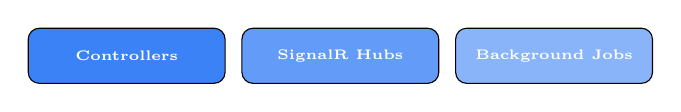
\begin{tikzpicture}[node distance=0.5cm]
    \node[block, fill=secondary, minimum width=2.5cm, minimum height=0.7cm, font=\tiny\bfseries] (ctl) {Controllers};
    \node[block, fill=secondary!80, right=0.2cm of ctl, minimum width=2.5cm, minimum height=0.7cm, font=\tiny\bfseries] (sgnlr) {SignalR Hubs};
    \node[block, fill=secondary!60, right=0.2cm of sgnlr, minimum width=2.5cm, minimum height=0.7cm, font=\tiny\bfseries] (bg) {Background Jobs};
\end{tikzpicture}
};
\draw[arrow] (gateway.south) -- (backend.north);

% ── AI Service ──
\node[container, label={[anchor=south west]{}AI Service (FastAPI)}, right=4cm of backend] (ai) {

\begin{tikzpicture}[node distance=0.5cm]
    \node[block, fill=accent, minimum width=2.2cm, minimum height=0.7cm, font=\tiny\bfseries] (match) {Matching};
    \node[block, fill=accent!80, right=0.2cm of match, minimum width=2.2cm, minimum height=0.7cm, font=\tiny\bfseries] (fuzzy) {Fuzzy Search};
    \node[block, fill=accent!60, right=0.2cm of fuzzy, minimum width=2.2cm, minimum height=0.7cm, font=\tiny\bfseries] (fraud) {Fraud Detect};
\end{tikzpicture}
};
\draw[arrow] (backend.east) -- node[above, font=\small] {HTTP} (ai.west);
\draw[arrow] (ai.west) -- node[below, font=\small] {HTTP} (backend.east);

% ── Data Layer ──
\node[container, label={[anchor=south west]{}Data Layer}, below=1.5cm of backend] (data) {
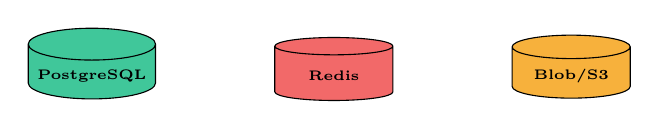
\begin{tikzpicture}[node distance=0.5cm]
    \node[db, fill=success!80, minimum width=1.5cm, minimum height=0.8cm, font=\tiny\bfseries] (pg) {PostgreSQL};
    \node[db, fill=danger!80, right=1.5cm of pg, minimum width=1.5cm, minimum height=0.8cm, font=\tiny\bfseries] (redis) {Redis};
    \node[db, fill=warning!80, right=1.5cm of redis, minimum width=1.5cm, minimum height=0.8cm, font=\tiny\bfseries] (blob) {Blob/S3};
\end{tikzpicture}
};
\draw[arrow] (backend.south) -- (data.north);
\draw[arrow] (ai.south) -- (data.north);

\end{tikzpicture}
\caption{\textbf{High-Level System Architecture --- Three-Service Topology}}
\label{fig:architecture}
\end{figure}

\section{Technology Stack}

\begin{longtable}{lll}
\toprule
\textbf{Layer} & \textbf{Technology} & \textbf{Rationale} \\
\midrule
\endhead
\bottomrule
\endfoot
Frontend       & Next.js 15 (App Router) + React 19 & SSR, SEO, file-based routing, React Server Components \\
Styling        & Tailwind CSS v4 + Motion (Framer Motion successor) & Utility-first, dark mode, animation primitives \\
Components     & shadcn/ui + Magic UI (extracted) & 150+ animated components, accessible, award-winning UI \\
State          & Zustand + TanStack Query & Client state + server cache with deduplication \\
Forms          & React Hook Form + Zod & Performant forms with schema validation \\
Backend        & ASP.NET Core 9 Web API & High-performance, strongly typed, native SignalR \\
ORM            & Entity Framework Core 9 & Mature, LINQ provider, migration tooling \\
Auth           & JWT Access + Refresh Token (HTTP-only cookies) & Stateless, secure, refresh rotation \\
Real-Time      & SignalR & Bidirectional, WebSocket with fallback transport \\
Cache          & Redis 7 & Low-latency, session store, pub/sub for SignalR \\
Database       & PostgreSQL 16 + pg\_trgm, CIText, UUIDv7 & JSONB, full-text search, trigram fuzzy matching \\
AI/ML Service  & FastAPI + scikit-learn & Async, auto-docs, simple regression/anomaly detection \\
Container      & Docker + Docker Compose & Reproducible environments, local dev parity \\
CI/CD          & GitHub Actions & Tight GitHub integration, matrix builds \\
\bottomrule
\end{longtable}

% ============================================================
\chapter{Role-Based Access Control}
% ============================================================

\section{RBAC Architecture}

\begin{figure}[H]
\centering
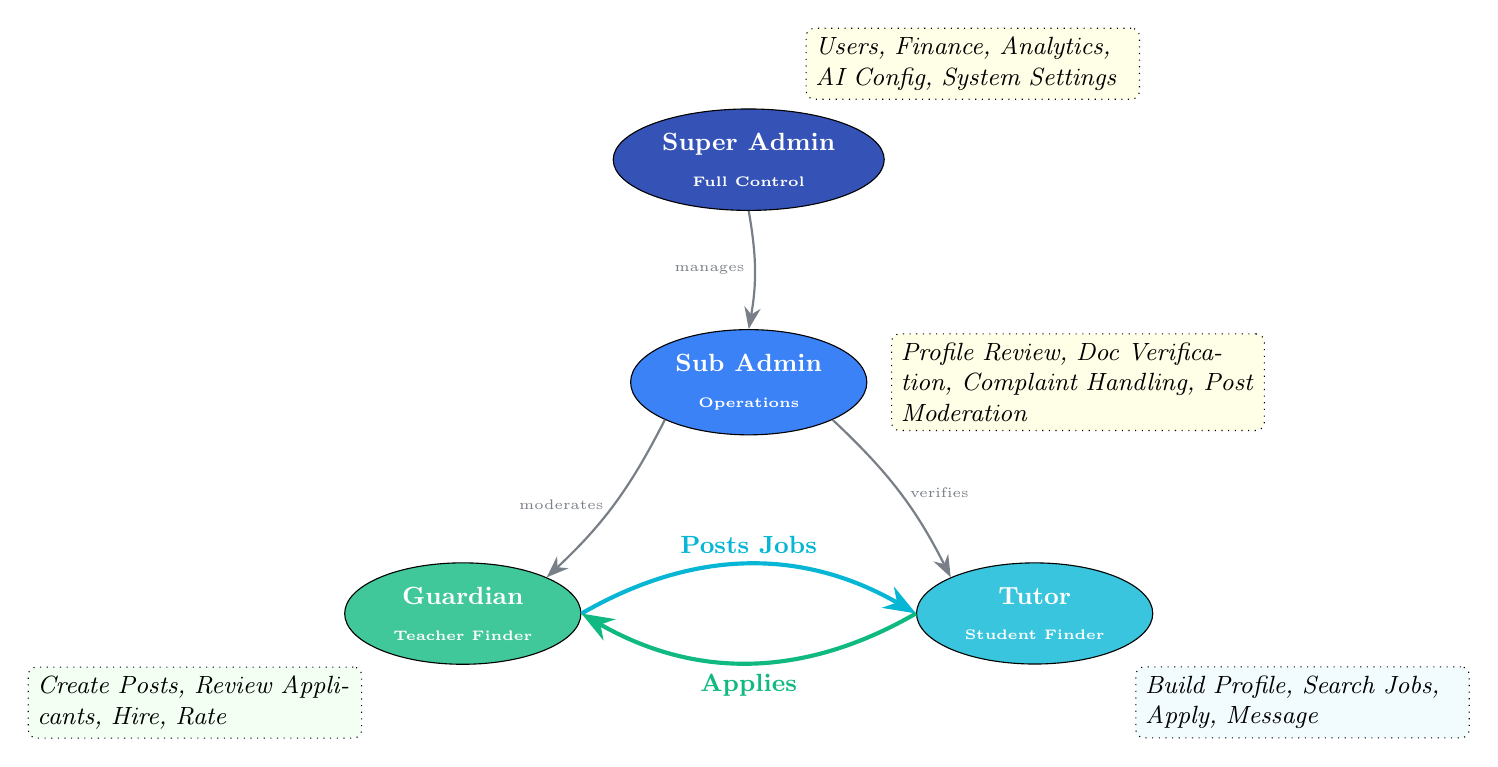
\begin{tikzpicture}[node distance=1.8cm]

% Roles
\node[role, fill=primary!90, text=white, minimum width=3cm] (super) {\textbf{Super Admin}\\[2pt]\tiny Full Control};
\node[role, fill=secondary, text=white, minimum width=3cm, below=1.5cm of super] (sub) {\textbf{Sub Admin}\\[2pt]\tiny Operations};
\node[role, fill=success!80, text=white, minimum width=3cm, below left=2cm and 1.5cm of sub] (guardian) {\textbf{Guardian}\\[2pt]\tiny Teacher Finder};
\node[role, fill=accent!80, text=white, minimum width=3cm, below right=2cm and 1.5cm of sub] (tutor) {\textbf{Tutor}\\[2pt]\tiny Student Finder};

% Hierarchical lines
\draw[arrow, bend left=10] (super.south) to node[left, font=\tiny] {manages} (sub.north);
\draw[arrow, bend left=10] (sub.south west) to node[left, font=\tiny] {moderates} (guardian.north east);
\draw[arrow, bend left=10] (sub.south east) to node[right, font=\tiny] {verifies} (tutor.north west);

% Marketplace flow
\draw[arrow, bend left=30, color=accent, line width=1.5pt] (guardian.east) to node[above, font=\small] {\textbf{Posts Jobs}} (tutor.west);
\draw[arrow, bend left=30, color=success, line width=1.5pt] (tutor.west) to node[below, font=\small] {\textbf{Applies}} (guardian.east);

% Permission annotations
\node[note, above right=0.3cm and -0.5cm of super, text width=4cm] {Users, Finance, Analytics, AI Config, System Settings};
\node[note, right=0.3cm of sub, text width=4.5cm] {Profile Review, Doc Verification, Complaint Handling, Post Moderation};
\node[note, below left=0.3cm of guardian, text width=4cm, fill=green!5] {Create Posts, Review Applicants, Hire, Rate};
\node[note, below right=0.3cm of tutor, text width=4cm, fill=cyan!5] {Build Profile, Search Jobs, Apply, Message};

\end{tikzpicture}
\caption{\textbf{Role Hierarchy \& Permission Boundaries}}
\end{figure}

\section{Permissions Matrix}

\begin{longtable}{p{4cm}|c|c|c|c}
\toprule
\textbf{Capability} & \textbf{Super Admin} & \textbf{Sub Admin} & \textbf{Guardian} & \textbf{Tutor} \\
\midrule
\endhead
\bottomrule
\endfoot
Manage Users             & \checkmark & \checkmark & --- & --- \\
Verify Tutors/Documents  & \checkmark & \checkmark & --- & --- \\
View Financial Reports   & \checkmark & --- & --- & --- \\
Configure Commission     & \checkmark & --- & --- & --- \\
Access Audit Logs        & \checkmark & \checkmark* & --- & --- \\
Handle Complaints        & \checkmark & \checkmark & File only & File only \\
Approve Tuition Posts    & \checkmark & \checkmark & --- & --- \\
Create Tuition Posts     & --- & --- & \checkmark & --- \\
Browse \& Apply Jobs     & --- & --- & --- & \checkmark \\
Hire/Reject Tutors       & --- & --- & \checkmark & --- \\
Rate \& Review           & --- & --- & \checkmark & --- \\
Live Chat                & --- & --- & \checkmark & \checkmark \\
View AI Insights         & \checkmark & \checkmark & Dashboard & Dashboard \\
Manage System Config     & \checkmark & --- & --- & --- \\
\bottomrule
\multicolumn{5}{l}{\tiny* Sub Admin: limited to operations-related logs only} \\
\end{longtable}

% ============================================================
\chapter{Database Schema}
% ============================================================

\section{Entity Relationship Diagram}

\begin{figure}[H]
\centering
\resizebox{\textwidth}{!}{%
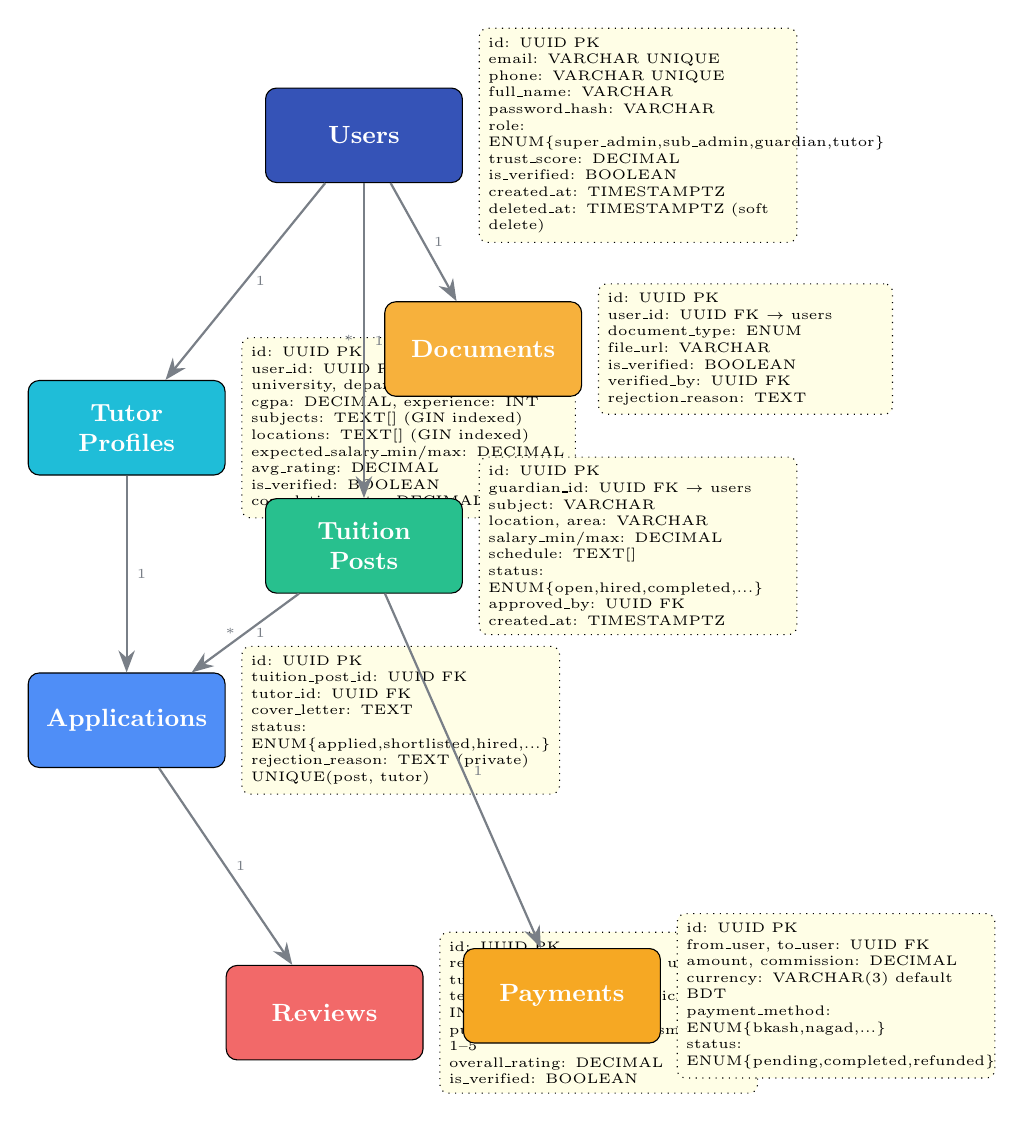
\begin{tikzpicture}[node distance=1.8cm, every node/.style={font=\small}]

% ── Users ──
\node[block, fill=primary!90, minimum width=2.5cm, minimum height=1.2cm] (users) {Users};
\node[note, right=0.2cm of users, text width=3.8cm, font=\tiny] {
    id: UUID PK\\
    email: VARCHAR UNIQUE\\
    phone: VARCHAR UNIQUE\\
    full\_name: VARCHAR\\
    password\_hash: VARCHAR\\
    role: ENUM\{super\_admin,sub\_admin,guardian,tutor\}\\
    trust\_score: DECIMAL\\
    is\_verified: BOOLEAN\\
    created\_at: TIMESTAMPTZ\\
    deleted\_at: TIMESTAMPTZ (soft delete)
};

% ── Tutor Profiles ──
\node[block, fill=accent!90, minimum width=2.5cm, minimum height=1.2cm, below left=2.5cm and 0.5cm of users] (tutor_profiles) {Tutor\\Profiles};
\node[note, right=0.2cm of tutor_profiles, text width=4cm, font=\tiny] {
    id: UUID PK\\
    user\_id: UUID FK $\to$ users\\
    university, department: VARCHAR\\
    cgpa: DECIMAL, experience: INT\\
    subjects: TEXT[] (GIN indexed)\\
    locations: TEXT[] (GIN indexed)\\
    expected\_salary\_min/max: DECIMAL\\
    avg\_rating: DECIMAL\\
    is\_verified: BOOLEAN\\
    completion\_rate: DECIMAL
};

% ── Documents ──
\node[block, fill=warning!80, minimum width=2.5cm, minimum height=1.2cm, below right=1.5cm and -1cm of users] (documents) {Documents};
\node[note, right=0.2cm of documents, text width=3.5cm, font=\tiny] {
    id: UUID PK\\
    user\_id: UUID FK $\to$ users\\
    document\_type: ENUM\\
    file\_url: VARCHAR\\
    is\_verified: BOOLEAN\\
    verified\_by: UUID FK\\
    rejection\_reason: TEXT
};

% ── Tuition Posts ──
\node[block, fill=success!90, minimum width=2.5cm, minimum height=1.2cm, below=4cm of users] (posts) {Tuition\\Posts};
\node[note, right=0.2cm of posts, text width=3.8cm, font=\tiny] {
    id: UUID PK\\
    guardian\_id: UUID FK $\to$ users\\
    subject: VARCHAR\\
    location, area: VARCHAR\\
    salary\_min/max: DECIMAL\\
    schedule: TEXT[]\\
    status: ENUM\{open,hired,completed,...\}\\
    approved\_by: UUID FK\\
    created\_at: TIMESTAMPTZ
};

% ── Applications ──
\node[block, fill=secondary!90, minimum width=2.5cm, minimum height=1.2cm, below=2.5cm of tutor_profiles] (applications) {Applications};
\node[note, right=0.2cm of applications, text width=3.8cm, font=\tiny] {
    id: UUID PK\\
    tuition\_post\_id: UUID FK\\
    tutor\_id: UUID FK\\
    cover\_letter: TEXT\\
    status: ENUM\{applied,shortlisted,hired,...\}\\
    rejection\_reason: TEXT (private)\\
    UNIQUE(post, tutor)
};

% ── Reviews ──
\node[block, fill=danger!80, minimum width=2.5cm, minimum height=1.2cm, below right=2.5cm and 0cm of applications] (reviews) {Reviews};
\node[note, right=0.2cm of reviews, text width=3.8cm, font=\tiny] {
    id: UUID PK\\
    reviewer\_id: UUID FK $\to$ users\\
    tutor\_id: UUID FK\\
    teaching\_quality, communication: INT 1--5\\
    punctuality, professionalism: INT 1--5\\
    overall\_rating: DECIMAL\\
    is\_verified: BOOLEAN
};

% ── Payments ──
\node[block, fill=warning!90, minimum width=2.5cm, minimum height=1.2cm, below right=4.5cm and 0cm of posts] (payments) {Payments};
\node[note, right=0.2cm of payments, text width=3.8cm, font=\tiny] {
    id: UUID PK\\
    from\_user, to\_user: UUID FK\\
    amount, commission: DECIMAL\\
    currency: VARCHAR(3) default BDT\\
    payment\_method: ENUM\{bkash,nagad,...\}\\
    status: ENUM\{pending,completed,refunded\}
};

% ── Relationships ──
\draw[arrow] (users) -- node[right, font=\tiny] {1} (tutor_profiles);
\draw[arrow] (users) -- node[right, font=\tiny] {1} (documents);
\draw[arrow] (users) -- node[right, font=\tiny] {1} node[left, font=\tiny] {*} (posts);
\draw[arrow] (posts) -- node[right, font=\tiny] {1} node[left, font=\tiny] {*} (applications);
\draw[arrow] (tutor_profiles) -- node[right, font=\tiny] {1} (applications);
\draw[arrow] (applications) -- node[right, font=\tiny] {1} (reviews);
\draw[arrow] (posts) -- node[right, font=\tiny] {1} (payments);

\end{tikzpicture}
}
\caption{\textbf{Core Entity Relationship Diagram (Simplified)}}
\label{fig:er-diagram}
\end{figure}

\section{Complete Schema Listing}

The full schema includes 13 tables:

\begin{longtable}{p{3.5cm}|p{3cm}|p{7cm}}
\toprule
\textbf{Table} & \textbf{Key Indexes} & \textbf{Purpose} \\
\midrule
\endhead
\bottomrule
\endfoot
users            & role, phone, trust\_score DESC & Platform users, authentication, role assignment \\
refresh\_tokens  & (user\_id), expires\_at WHERE revoked & Secure JWT refresh token rotation \\
otp\_codes       & (user\_id, type) & Email/phone verification, password reset \\
tutor\_profiles  & is\_verified, avg\_rating DESC, GIN(subjects, locations) & Extended tutor profile, search, matching \\
documents        & user\_id, is\_verified & Verification document storage \\
tuition\_posts   & guardian\_id, status(open), subject, location, salary & Job listings with full-text search \\
applications     & (post\_id, tutor\_id), status & Job application workflow \\
reviews          & tutor\_id, overall\_rating DESC & Multi-factor tutor rating system \\
guardian\_verifications & user\_id, verification\_level, is\_verified & Guardian NID/phone verification \\
payment\_transactions & from\_user, to\_user, status & Revenue, commission, payouts \\
conversations / messages & (conversation\_id, created\_at), unread filter & Real-time chat \\
notifications    & (user\_id, is\_read, created\_at DESC) & In-app + push notifications \\
audit\_logs      & user\_id, action, (entity\_type, entity\_id) & Compliance, monitoring \\
guardian\_verifications & user\_id, verification\_level, is\_verified & Guardian NID/phone/email verification \\
system\_config   & key UNIQUE & Dynamic configuration (commission, weights) \\
\bottomrule
\end{longtable}

\section{Key Indexing Strategy}

\begin{longtable}{p{4cm}|p{2.5cm}|p{7cm}}
\toprule
\textbf{Query Pattern} & \textbf{Index Type} & \textbf{Details} \\
\midrule
\endhead
\bottomrule
\endfoot
Browse open tuition posts          & Partial B-tree   & WHERE status = 'open' ORDER BY created\_at DESC \\
Fuzzy search subjects/locations    & GIN trigram       & pg\_trgm extension, similarity() function \\
Tutor recommendations              & Multi-column      & avg\_rating DESC, trust\_score DESC, total\_hires DESC \\
Search tutors by subject/location  & GIN array         & teaching\_subjects[], preferred\_locations[] \\
Guardian's active posts            & Composite B-tree  & (guardian\_id, status) \\
Unread notifications               & Partial B-tree    & (user\_id, is\_read) WHERE is\_read = FALSE \\
Active complaints                  & Partial B-tree    & status WHERE status IN ('open', 'investigating') \\
Payment history                    & B-tree            & from\_user\_id, to\_user\_id, created\_at DESC \\
Chat messages                      & Composite B-tree  & (conversation\_id, created\_at) \\
\bottomrule
\end{longtable}

% ============================================================
\chapter{Backend Architecture}
% ============================================================

\section{Clean Architecture Layers}

\begin{figure}[H]
\centering
\begin{tikzpicture}[
    every node/.style={align=center},
    layer/.style={rectangle, draw, rounded corners=6pt, minimum width=10cm, font=\large\bfseries},
    comp/.style={rectangle, draw, fill=white, rounded corners=3pt, minimum width=2.8cm, minimum height=0.6cm, font=\small}
]

% ── Domain Layer ──
\node[layer, fill=green!15, draw=green!50!black, minimum height=2.8cm] (domain) {
    \textbf{TuitionHub.Domain}\\[6pt]
    \begin{tikzpicture}
        \node[comp] (d1) {Entities};
        \node[comp, right=0.3cm of d1] (d2) {Value Objects};
        \node[comp, below=0.3cm of d1] (d3) {Domain Interfaces};
        \node[comp, right=0.3cm of d3] (d4) {Domain Exceptions};
    \end{tikzpicture}
};

% ── Application Layer ──
\node[layer, fill=blue!10, draw=blue!50!black, minimum height=2.8cm, above=0.6cm of domain] (app) {
    \textbf{TuitionHub.Application}\\[6pt]
    \begin{tikzpicture}
        \node[comp] (a1) {Commands / Queries};
        \node[comp, right=0.3cm of a1] (a2) {Handlers (MediatR)};
        \node[comp, below=0.3cm of a1] (a3) {DTOs + Mappings};
        \node[comp, right=0.3cm of a3] (a4) {Behaviors (Pipeline)};
    \end{tikzpicture}
};
\draw[arrow, bend right=8] (domain.north) to node[right, font=\tiny] {depends only} (app.south);

% ── Infrastructure Layer ──
\node[layer, fill=orange!10, draw=orange!50!black, minimum height=2.8cm, above=0.6cm of app] (infra) {
    \textbf{TuitionHub.Infrastructure}\\[6pt]
    \begin{tikzpicture}
        \node[comp] (i1) {EF Core DbContext};
        \node[comp, below=0.25cm of i1] (i2) {Repositories};
        \node[comp, below=0.25cm of i2] (i3) {Identity + JWT};
        \node[comp, right=0.3cm of i1] (i4) {Email / SMS / File};
        \node[comp, below=0.25cm of i4] (i5) {SignalR Hubs};
        \node[comp, below=0.25cm of i5] (i6) {Redis Cache};
    \end{tikzpicture}
};
\draw[arrow, bend right=8] (app.north) to node[right, font=\tiny] {depends only} (infra.south);

% ── API Layer ──
\node[layer, fill=purple!10, draw=purple!50!black, minimum height=2.8cm, above=0.6cm of infra] (api) {
    \textbf{TuitionHub.Api}\\[6pt]
    \begin{tikzpicture}
        \node[comp] (p1) {Controllers};
        \node[comp, right=0.3cm of p1] (p2) {Middleware};
        \node[comp, below=0.3cm of p1] (p3) {Hubs};
        \node[comp, right=0.3cm of p3] (p4) {Filters};
    \end{tikzpicture}
};
\draw[arrow, bend right=8] (infra.north) to node[right, font=\tiny] {depends only} (api.south);

\end{tikzpicture}
\caption{\textbf{Clean Architecture --- Dependency Inversion Principle}}
\label{fig:clean-arch}
\end{figure}

\section{CQRS with MediatR}

Each use case is represented as a \texttt{Command} (write) or \texttt{Query} (read), handled through MediatR with pipeline behaviors for cross-cutting concerns:

\begin{figure}[H]
\centering
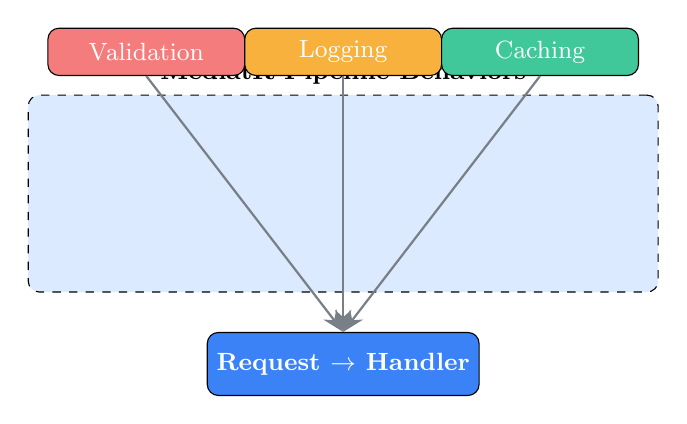
\begin{tikzpicture}[node distance=0.8cm]
\node[rectangle, draw, dashed, rounded corners=4pt, fill=blueprint, minimum width=8cm, minimum height=2.5cm] (pipeline) {};
\node[above] at (pipeline.north) {\small\textbf{MediatR Pipeline Behaviors}};
\node[block, fill=danger!70, minimum width=2.5cm, minimum height=0.6cm, font=\small] (val) at (-2.5,1.8) {Validation};
\node[block, fill=warning!80, minimum width=2.5cm, minimum height=0.6cm, font=\small] (log) at (0,1.8) {Logging};
\node[block, fill=success!80, minimum width=2.5cm, minimum height=0.6cm, font=\small] (cache) at (2.5,1.8) {Caching};
\node[block, fill=secondary, minimum width=3cm, minimum height=0.8cm, below=0.5cm of pipeline] (request) {Request $\to$ Handler};
\draw[arrow] (val.south) -- (request.north);
\draw[arrow] (log.south) -- (request.north);
\draw[arrow] (cache.south) -- (request.north);
\end{tikzpicture}
\caption{\textbf{MediatR Pipeline with Cross-Cutting Behaviors}}
\end{figure}

\section{JWT Authentication Flow}

\begin{figure}[H]
\centering
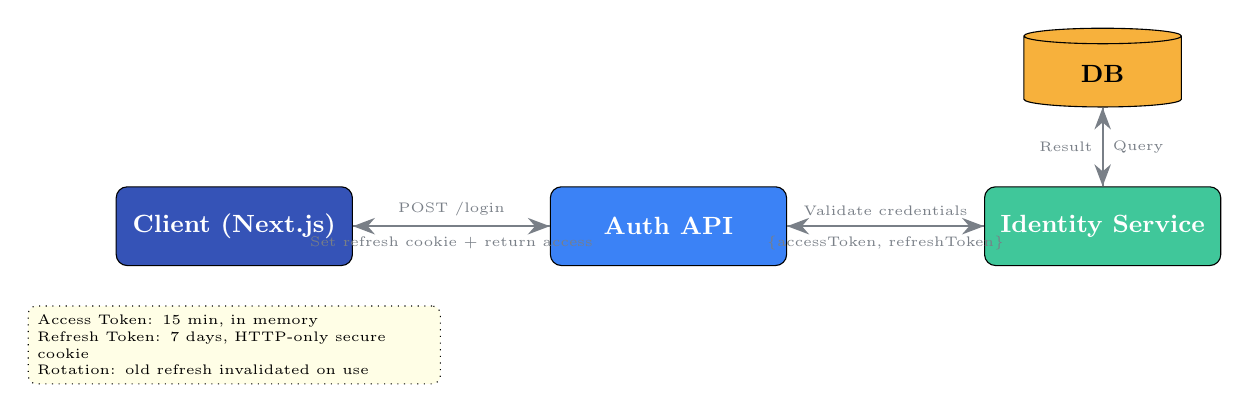
\begin{tikzpicture}[node distance=1.5cm]

\node[block, fill=primary!90, minimum width=3cm] (client) {Client (Next.js)};
\node[block, fill=secondary, right=2.5cm of client, minimum width=3cm] (api) {Auth API};
\node[block, fill=success!80, right=2.5cm of api, minimum width=3cm] (identity) {Identity Service};
\node[db, fill=warning!80, above=1cm of identity] (db) {DB};

\draw[arrow] (client.east) -- node[above, font=\tiny] {POST /login} (api.west);
\draw[arrow] (api.east) -- node[above, font=\tiny] {Validate credentials} (identity.west);
\draw[arrow, bend left=20] (identity.north) -- node[right, font=\tiny] {Query} (db.south);
\draw[arrow, bend left=20] (db.south) -- node[left, font=\tiny] {Result} (identity.north);

\draw[arrow] (identity.west) -- node[below, font=\tiny] {\{accessToken, refreshToken\}} (api.east);
\draw[arrow] (api.west) -- node[below, font=\tiny] {Set refresh cookie + return access} (client.east);

\node[note, below=0.5cm of client, text width=5cm, font=\tiny] {
    Access Token: 15 min, in memory\\
    Refresh Token: 7 days, HTTP-only secure cookie\\
    Rotation: old refresh invalidated on use
};

\end{tikzpicture}
\caption{\textbf{JWT Access + Refresh Token Architecture}}
\end{figure}

% ============================================================
\chapter{Frontend Architecture}
% ============================================================

\section{Component Architecture}

\begin{figure}[H]
\centering
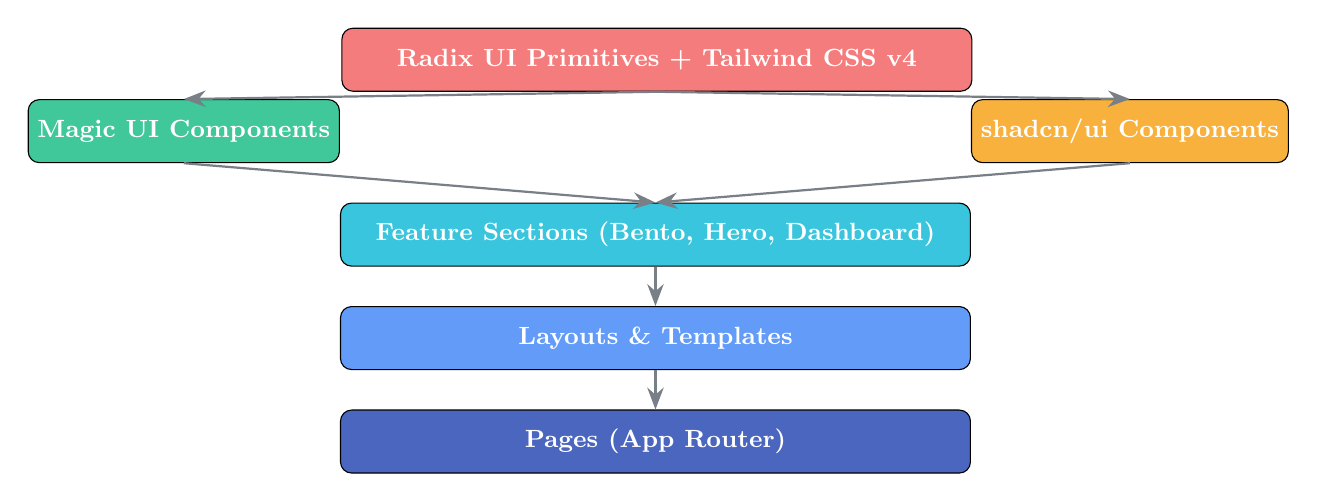
\begin{tikzpicture}[node distance=0.8cm]

\node[block, fill=primary!80, minimum width=8cm, minimum height=0.8cm] (pages) {Pages (App Router)};

\node[block, fill=secondary!80, minimum width=8cm, minimum height=0.8cm, above=0.5cm of pages] (layout) {Layouts \& Templates};

\node[block, fill=accent!80, minimum width=8cm, minimum height=0.8cm, above=0.5cm of layout] (sections) {Feature Sections (Bento, Hero, Dashboard)};

\node[block, fill=success!80, minimum width=3.5cm, minimum height=0.8cm, above left=0.5cm and 0cm of sections] (magicui) {Magic UI Components};
\node[block, fill=warning!80, minimum width=3.5cm, minimum height=0.8cm, above right=0.5cm and 0cm of sections] (shadcn) {shadcn/ui Components};

\node[block, fill=danger!70, minimum width=8cm, minimum height=0.8cm, above=0.5cm of $(magicui)!0.5!(shadcn)$] (primitives) {Radix UI Primitives + Tailwind CSS v4};

\draw[arrow] (primitives.south) -- (magicui.north);
\draw[arrow] (primitives.south) -- (shadcn.north);
\draw[arrow] (magicui.south) -- (sections.north);
\draw[arrow] (shadcn.south) -- (sections.north);
\draw[arrow] (sections.south) -- (layout.north);
\draw[arrow] (layout.south) -- (pages.north);

\end{tikzpicture}
\caption{\textbf{Frontend Component Hierarchy}}
\end{figure}

\section{Route Structure}

\begin{longtable}{p{1.5cm}|p{3.5cm}|p{3cm}|p{5cm}}
\toprule
\textbf{Group} & \textbf{Routes} & \textbf{Access} & \textbf{Content} \\
\midrule
\endhead
\bottomrule
\endfoot
Marketing & /, /about, /pricing, /contact & Public & Landing page (Magic UI hero, bento, marquee), SEO-optimized \\
Auth      & /login, /register, /forgot-password, /verify-otp & Public & Forms with Zod validation, OTP input, password strength \\
Jobs      & /jobs, /jobs/[id] & All & Tuition listing with fuzzy search, filters, pagination \\
Tutors    & /tutors, /tutors/[id] & All & Tutor search with matching score badges, profiles \\
Guardian  & /dashboard/guardian/* & Guardian only & Posts CRUD, applicants, hires, reviews, chat \\
Tutor     & /dashboard/tutor/* & Tutor only & Profile, applications, job search, reviews, chat \\
Admin     & /dashboard/admin/* & Super/Sub Admin & User mgmt, verifications, finance, analytics, complaints \\
\bottomrule
\end{longtable}

% ============================================================
\chapter{Matching Engine \& Search}
% ============================================================

\section{Tutor Matching Algorithm}

The matching engine is a \textbf{pure rule-based scorer} with configurable weights stored in the database (system\_config table). No LLM, no neural networks.

\begin{figure}[H]
\centering
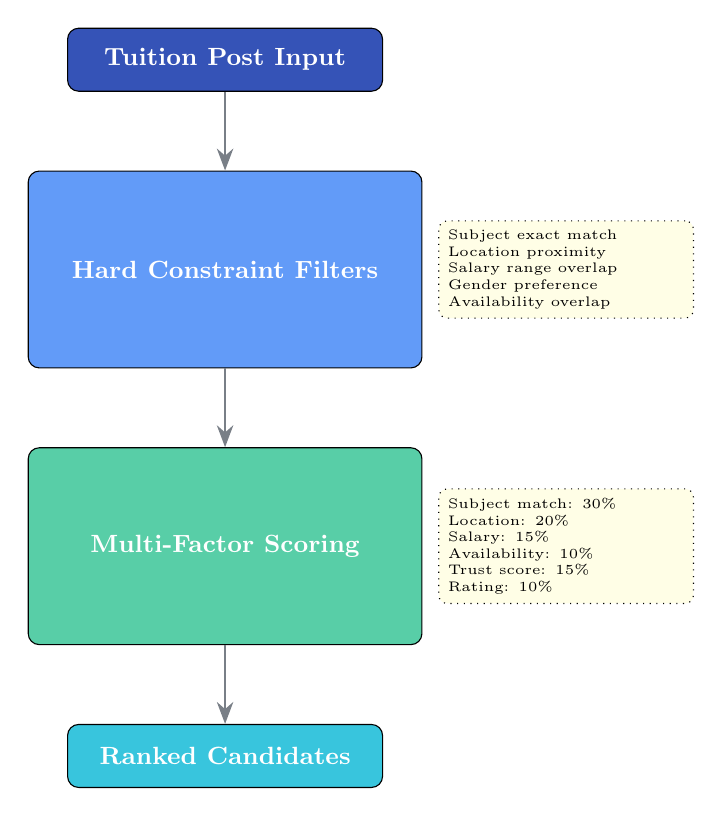
\begin{tikzpicture}[node distance=1.2cm]

\node[block, fill=primary!90, minimum width=4cm, minimum height=0.8cm] (post) {Tuition Post Input};

\node[block, fill=secondary!80, minimum width=5cm, minimum height=2.5cm, below=1cm of post] (filters) {Hard Constraint Filters};
\node[note, right=0.2cm of filters, text width=3cm, font=\tiny] {
    Subject exact match\\
    Location proximity\\
    Salary range overlap\\
    Gender preference\\
    Availability overlap
};

\node[block, fill=success!70, minimum width=5cm, minimum height=2.5cm, below=1cm of filters] (scoring) {Multi-Factor Scoring};
\node[note, right=0.2cm of scoring, text width=3cm, font=\tiny] {
    Subject match: 30\%\\
    Location: 20\%\\
    Salary: 15\%\\
    Availability: 10\%\\
    Trust score: 15\%\\
    Rating: 10\%
};

\node[block, fill=accent!80, minimum width=4cm, minimum height=0.8cm, below=1cm of scoring] (ranked) {Ranked Candidates};

\draw[arrow] (post.south) -- (filters.north);
\draw[arrow] (filters.south) -- (scoring.north);
\draw[arrow] (scoring.south) -- (ranked.north);

\end{tikzpicture}
\caption{\textbf{Matching Pipeline --- Constraints $\to$ Scoring $\to$ Ranking}}
\label{fig:matching}
\end{figure}

\subsection{Scoring Formula}
\begin{verbatim}
Score = subject_match * 0.30 +
        location_match * 0.20 +
        salary_overlap * 0.15 +
        availability_overlap * 0.10 +
        (trust_score / 5.0) * 0.15 +
        (avg_rating / 5.0) * 0.10
\end{verbatim}

All weights are configurable by Super Admin via the system\_config table, allowing dynamic tuning without code deployment.

\section{Fuzzy Search Implementation}

PostgreSQL \texttt{pg\_trgm} extension provides trigram-based fuzzy matching:

\begin{itemize}
    \item \textbf{Trigram Index}: All subject names, locations, and post titles are decomposed into 3-character sequences
    \item \textbf{Similarity Operator} (\texttt{\%}): Returns results where trigram similarity exceeds threshold
    \item \textbf{Distance Function} (\texttt{<->}): Used for sorting by closest match
    \item Works for both \textbf{Bangla and English} text
\end{itemize}

\begin{lstlisting}[style=code, language=SQL, caption={Fuzzy Search Query Example}]
-- Enable extension
CREATE EXTENSION IF NOT EXISTS pg_trgm;

-- Trigram index on searchable fields
CREATE INDEX idx_posts_title_trgm ON tuition_posts 
    USING GIN (title gin_trgm_ops);
CREATE INDEX idx_posts_subject_trgm ON tuition_posts 
    USING GIN (subject gin_trgm_ops);
CREATE INDEX idx_posts_location_trgm ON tuition_posts 
    USING GIN (location gin_trgm_ops);

-- Fuzzy search with ranking
SELECT id, title, subject, location, 
       similarity(title, 'math ttor') AS sim_score
FROM tuition_posts
WHERE status = 'open'
  AND (title % 'math ttor' OR subject % 'math')
  AND location % 'dhanmondi'
ORDER BY sim_score DESC
LIMIT 20;
\end{lstlisting}

\section{Salary Prediction}

A \textbf{linear regression model} (scikit-learn) trained on historical completed hire data:

\begin{lstlisting}[style=code, language=Python, caption={Salary Prediction Model}]
import sklearn.linear_model
import numpy as np

# Features: subject_encoded, location_encoded, class_grade,
#           tutor_experience, tutor_cgpa, teaching_medium
model = sklearn.linear_model.LinearRegression()
model.fit(X_train, y_train)  # trained on completed hires

def predict_salary(features: dict) -> dict:
    X = np.array([[features['subject_enc'], features['location_enc'],
                   features['grade_enc'], features['experience'],
                   features['cgpa'], features['medium_enc']]])
    predicted = model.predict(X)[0]
    return {
        'predicted_min': round(predicted * 0.8),
        'predicted_max': round(predicted * 1.2),
        'recommended': round(predicted),
        'confidence': model.score(X_test, y_test)
    }
\end{lstlisting}

\section{Fraud Detection}

Hybrid approach: \textbf{rule-based scoring} + \textbf{Isolation Forest} anomaly detection:

\begin{lstlisting}[style=code, language=Python, caption={Fraud Risk Score Calculation}]
def fraud_risk_score(profile: dict, behavior: dict) -> dict:
    risk = 0
    
    # Rule-based checks
    if profile.get('age', 0) < 18: risk += 25
    if profile.get('university') == '': risk += 10
    if not profile.get('documents_submitted'): risk += 20
    if behavior.get('login_frequency', 0) > 100: risk += 15
    if behavior.get('device_count', 0) > 3: risk += 10
    
    # Anomaly detection (Isolation Forest)
    features = np.array([[...features...]])
    anomaly_score = isolation_forest.decision_function(features)
    if anomaly_score < -0.5: risk += 20  # outlier detected
    
    # Classification
    if risk < 30:       level = 'low'
    elif risk < 60:     level = 'medium'
    else:               level = 'high'
    
    return {'risk_score': risk, 'risk_level': level}
\end{lstlisting}

\section{Trust Score Calculation}

\begin{verbatim}
trust_score = (
    (avg_rating / 5.0) * 0.30 +          # rating contribution
    completion_rate * 0.20 +              # completed / hired
    normalized_response_time * 0.10 +     # faster = higher score
    log_scale(total_hires) * 0.10 +       # experience
    profile_completeness * 0.10 +          # % of fields filled
    (1.0 if verified else 0.3) * 0.10 +   # verification bonus
    (1.0 - complaint_penalty) * 0.10       # complaint deduction
) * 5.0  # scale to 5.0
\end{verbatim}

% ============================================================
\chapter{API Design}
% ============================================================

\section{API Response Envelope}
\begin{lstlisting}[style=code, language=TeX, caption={Standard API Response (JSON)}]
{
    "success": true,
    "data": { ... },
    "message": "Operation completed successfully",
    "errors": [],
    "meta": {
        "page": 1,
        "pageSize": 20,
        "totalCount": 150,
        "totalPages": 8
    }
}
\end{lstlisting}

\section{API Endpoint Map}

\begin{longtable}{p{1.5cm}|p{6cm}|p{6cm}}
\toprule
\textbf{Method} & \textbf{Endpoint} & \textbf{Description} \\
\midrule
\endhead
\bottomrule
\endfoot
\multicolumn{3}{l}{\textbf{Authentication}} \\
POST & /api/v1/auth/register & Register guardian or tutor \\
POST & /api/v1/auth/login & Login $\to$ JWT access + refresh token \\
POST & /api/v1/auth/refresh & Rotate refresh token \\
POST & /api/v1/auth/verify-otp & Verify email/phone via OTP \\
POST & /api/v1/auth/forgot-password & Send password reset OTP \\
POST & /api/v1/auth/reset-password & Reset password with OTP \\

\multicolumn{3}{l}{\textbf{Users}} \\
GET  & /api/v1/users/me & Current user profile \\
PUT  & /api/v1/users/me & Update profile \\
POST & /api/v1/users/me/documents & Upload verification documents \\
GET  & /api/v1/users/\{id\} & Public user profile \\

\multicolumn{3}{l}{\textbf{Tutors}} \\
GET  & /api/v1/tutors & Search/filter tutors with fuzzy search \\
GET  & /api/v1/tutors/\{id\} & Tutor public profile with rating \\
GET  & /api/v1/tutors/\{id\}/reviews & Paginated tutor reviews \\
POST & /api/v1/tutors/recommendations & AI-matched tutor recommendations \\

\multicolumn{3}{l}{\textbf{Tuition Posts}} \\
GET  & /api/v1/tuition-posts & Browse with fuzzy search, filters, pagination \\
POST & /api/v1/tuition-posts & Guardian creates tuition post \\
PUT  & /api/v1/tuition-posts/\{id\} & Update post \\
PATCH & /api/v1/tuition-posts/\{id\}/status & Change post status \\
DELETE & /api/v1/tuition-posts/\{id\} & Soft-delete post \\

\multicolumn{3}{l}{\textbf{Applications}} \\
POST & /api/v1/applications & Tutor applies to tuition post \\
GET  & /api/v1/applications & List applications (filter by user/post) \\
PATCH & /api/v1/applications/\{id\}/shortlist & Guardian shortlists \\
PATCH & /api/v1/applications/\{id\}/hire & Guardian hires \\
PATCH & /api/v1/applications/\{id\}/reject & Guardian rejects with private feedback \\

\multicolumn{3}{l}{\textbf{Reviews}} \\
POST & /api/v1/reviews & Create multi-factor review \\
GET  & /api/v1/reviews & List reviews (filter by tutor) \\
PATCH & /api/v1/reviews/\{id\}/flag & Admin flags suspicious review \\

\multicolumn{3}{l}{\textbf{Payments}} \\
POST & /api/v1/payments/commission & Calculate commission \\
GET  & /api/v1/payments/transactions & Payment history \\
GET  & /api/v1/payments/reports & Admin revenue reports \\

\multicolumn{3}{l}{\textbf{Chat}} \\
GET  & /api/v1/chat/conversations & List conversations \\
POST & /api/v1/chat/conversations & Create conversation \\
GET  & /api/v1/chat/conversations/\{id\}/messages & Message history \\
POST & /api/v1/chat/conversations/\{id\}/messages & Send message \\
\multicolumn{3}{l}{\textbf{Admin}} \\
GET  & /api/v1/admin/dashboard & Aggregated statistics \\
GET  & /api/v1/admin/users & User management list \\
PATCH & /api/v1/admin/users/\{id\}/verify & Verify tutor \\
DELETE & /api/v1/admin/users/\{id\} & Suspend/ban user \\
GET  & /api/v1/admin/audit-logs & Compliance audit \\
GET  & /api/v1/admin/reports/\{type\} & Business reports \\
\bottomrule
\end{longtable}

% ============================================================
\chapter{Business Model \& Monetization Strategy}
% ============================================================

\section{Proposed Model Overview}

\begin{longtable}{p{4cm}|p{4cm}|p{4cm}}
\toprule
\textbf{Revenue Stream} & \textbf{Who Pays} & \textbf{When} \\
\midrule
\endhead
\bottomrule
\endfoot
Commission (30\% of 1st month salary) & Tutor & Upon successful hire \\
Registration Fee (BDT 500, one-time)   & Tutor & After free launch period \\
Premium Verified Badge (BDT 5,000)    & Tutor & Growth phase (eligibility-gated) \\
Freemium Guardian Features            & Guardian & Scale phase \\
Advertising \& Sponsorships           & Advertisers & Growth phase onward \\
\bottomrule
\end{longtable}

\section{Revenue Stream Analysis}

\subsection{Core: 30\% Commission on First Month's Salary}

\textbf{Target:} Tutors who get hired through the platform. \\
\textbf{Mechanism:} One-time deduction from the first month's tuition payment. No recurring fees. \\
\textbf{Rationale:} Aligns platform revenue with value delivered — tutor only pays when they actually get hired.

\begin{longtable}{p{4cm}|p{9cm}}
\toprule
\textbf{Dimension} & \textbf{Assessment} \\
\midrule
\endhead
\bottomrule
\endfoot
Advantages       & Low upfront barrier, highly scalable, perceived as fair (pay-per-success) \\
Disadvantages    & Revenue is delayed (only realized after hire), high rate (30\%) may incentivize platform bypass \\
Risk             & Tutors and guardians may attempt to connect once and transact offline \\
Mitigation       & In-app messaging enforced until hire confirmation. Contact info released only after commission recorded. \\
User Acceptance  & Moderate — tutors will compare with free Facebook groups, so value proposition must be clear \\
Implementation   & Phase 3 (MVP) — payment integration with bKash/Nagad \\
\bottomrule
\end{longtable}

\subsection{Registration Fee: BDT 500 (One-Time)}

\textbf{Target:} New tutors registering after the free launch period. \\
\textbf{Mechanism:} One-time payment to activate tutor account. \\
\textbf{Purpose:} Filters unserious applicants, generates baseline revenue, signals commitment.

\begin{longtable}{p{4cm}|p{9cm}}
\toprule
\textbf{Dimension} & \textbf{Assessment} \\
\midrule
\endhead
\bottomrule
\endfoot
Advantages       & Filters low-quality signups, generates early revenue,低廉 barrier relative to earning potential \\
Disadvantages    & May slow supply-side growth, creates friction for genuine but cash-strapped students \\
Risk             & Competitors offering free signups may capture market share \\
Mitigation       & Introduce only after critical mass of tuition posts exists (demand-pull justifies fee) \\
User Acceptance  & Low to moderate initially — requires strong value proposition \\
Implementation   & Phase 4 (Growth) — not during MVP \\
\bottomrule
\end{longtable}

\subsection{Premium Verified Badge: BDT 5,000}

\textbf{Target:} Tutors seeking higher visibility and credibility. \\
\textbf{Mechanism:} Eligibility-gated badge — the platform evaluates the tutor first, then allows purchase only if criteria are met. This is \textbf{not} pay-to-win.

\textbf{Eligibility Criteria:}
\begin{itemize}
    \item Identity verified (NID, student ID, or passport)
    \item Academic documents verified (transcript, certificate)
    \item Minimum trust score $\geq$ 4.0
    \item No unresolved complaints
    \item Minimum 3 completed tuition jobs
    \item Profile completeness $\geq$ 90\%
\end{itemize}

\textbf{Benefits:}
\begin{itemize}
    \item Priority placement in search results (boosted weight in matching engine)
    \item Featured on homepage tutor carousel
    \item Premium "Verified" badge on profile
    \item Higher visibility in recommendation engine
    \item Priority customer support
\end{itemize}

\begin{longtable}{p{4cm}|p{9cm}}
\toprule
\textbf{Dimension} & \textbf{Assessment} \\
\midrule
\endhead
\bottomrule
\endfoot
Advantages       & High-margin, builds trust ecosystem, incentivizes profile quality \\
Disadvantages    & Complex verification workflow, manual review overhead initially \\
Risk             & Perceived as elitist or unfair if criteria are unclear \\
Mitigation       & Transparent criteria published; Admin review + AI-assisted verification \\
User Acceptance  & High — tutors want trust signals to stand out \\
Implementation   & Phase 5 (Growth) — after stable marketplace exists \\
\bottomrule
\end{longtable}

\subsection{Freemium Guardian Features}

\textbf{Target:} Guardians posting tuition jobs. \\
\textbf{Free tier:} Post tuition jobs, review applicants, hire tutors, rate/review. \\
\textbf{Premium features (future):}
\begin{itemize}
    \item Featured/boosted tuition post (higher visibility to tutors)
    \item Urgent hiring package (express matching within 24 hours)
    \item Background check report on shortlisted tutors
    \item Priority customer support
\end{itemize}

\subsection{Secondary Revenue Streams (Growth \& Scale)}

\begin{longtable}{p{3.5cm}|p{2.5cm}|p{2.5cm}|p{4.5cm}}
\toprule
\textbf{Stream} & \textbf{Phase} & \textbf{Est. Complexity} & \textbf{Notes} \\
\midrule
\endhead
\bottomrule
\endfoot
Google AdSense / Display Ads    & Growth   & Low    & Non-intrusive banner ads on public pages \\
Sponsored Tutor Profiles        & Growth   & Medium & Premium placement in search results \\
Sponsored Tuition Posts         & Growth   & Medium & Guardian pays to boost post visibility \\
Affiliate Program (tutor referral) & Growth & Medium & Referral bonus for bringing new tutors \\
Recruitment Partnerships        & Scale    & High   & API/portal for coaching centers to bulk-hire \\
Digital Achievement Badges      & Growth   & Low    & Certificates for completed jobs,徽章 \\
Online Course Promotions        & Scale    & Medium & Partner with 10 Minute School, Shikho \\
Background Verification Service & Scale    & High   & Third-party verification for guardians too \\
\bottomrule
\end{longtable}

\section{Phased Monetization Roadmap}

\begin{figure}[H]
\centering
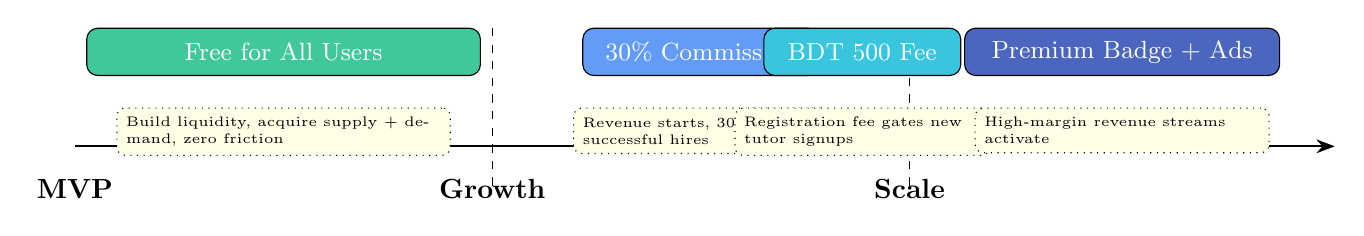
\begin{tikzpicture}[node distance=0.5cm]

% Timeline
\draw[thick, -{Stealth}] (0,0) -- (16,0);
\node[below] at (0,-0.3) {\textbf{MVP}};
\node[below] at (5.3,-0.3) {\textbf{Growth}};
\node[below] at (10.6,-0.3) {\textbf{Scale}};

% Phase markers
\draw[dashed] (5.3,-0.5) -- (5.3, 1.5);
\draw[dashed] (10.6,-0.5) -- (10.6, 1.5);

% Phase blocks (give each a name)
\node[block, fill=success!80, minimum width=5cm, minimum height=0.6cm, font=\small] (phase1) at (2.65,1.2) {Free for All Users};
\node[block, fill=secondary!80, minimum width=3cm, minimum height=0.6cm, font=\small] (phase2) at (7.95,1.2) {30\% Commission};
\node[block, fill=accent!80, minimum width=2.5cm, minimum height=0.6cm, font=\small] (phase3) at (10,1.2) {BDT 500 Fee};
\node[block, fill=primary!80, minimum width=4cm, minimum height=0.6cm, font=\small] (phase4) at (13.3,1.2) {Premium Badge + Ads};

% Annotations
\node[note, below=0.4cm of phase1.south, anchor=north, text width=4cm, font=\tiny] {Build liquidity, acquire supply + demand, zero friction};
\node[note, below=0.4cm of phase2.south, anchor=north, text width=3cm, font=\tiny] {Revenue starts, 30\% only on successful hires};
\node[note, below=0.4cm of phase3.south, anchor=north, text width=3cm, font=\tiny] {Registration fee gates new tutor signups};
\node[note, below=0.4cm of phase4.south, anchor=north, text width=3.5cm, font=\tiny] {High-margin revenue streams activate};

\end{tikzpicture}
\caption{\textbf{Monetization Phasing}}
\end{figure}

% ============================================================
\chapter{Go-to-Market Strategy}
% ============================================================

\section{The Chicken-and-Egg Problem}

Every marketplace faces this: \textbf{Tutors won't join without tuition posts; guardians won't post without tutors.} The solution is a \textbf{supply-first (tutor-first) acquisition strategy}, executed in phases.

\section{Phase 1: Supply-First (Dhaka Pilot — Months 0--2)}

\textbf{Strategy:} Recruit a critical mass of high-quality tutors before marketing to guardians.

\begin{longtable}{p{3cm}|p{10cm}}
\toprule
\textbf{Tactic} & \textbf{Execution} \\
\midrule
\endhead
\bottomrule
\endfoot
Campus Ambassador Program & Recruit 1 ambassador per major university (DU, BUET, JU, NSU, BRAC, etc.). Ambassadors get BDT 200 per verified tutor referral. \\
Free Profile Setup Drive & First 1,000 tutors get lifetime free profiles (grandfathered). Creates urgency. \\
University Partnerships & Partner with university career centers to promote the platform as a reliable tuition-finding tool. \\
Social Proof & Highlight top tutors from prestigious universities to attract both tutors and guardians. \\
Dhaka-Only Focus & All marketing and operations confined to Dhaka for measurable, concentrated growth. \\
Target: & \textbf{2,000+ verified tutors in Dhaka} before opening to guardians. \\
\bottomrule
\end{longtable}

\section{Phase 2: Demand Activation (Months 2--4)}

\textbf{Strategy:} Turn on guardian acquisition with a built-in tutor pool.

\begin{longtable}{p{3cm}|p{10cm}}
\toprule
\textbf{Tactic} & \textbf{Execution} \\
\midrule
\endhead
\bottomrule
\endfoot
Guardian Free Posting & Tuition posts are completely free. Zero friction to create a post. \\
Facebook Group Infiltration & Target the largest tuition-related Facebook groups (\"Tuition in Dhaka\", \"Tutor Wanted Bangladesh\") with targeted posts and ads. \\
Referral Incentive & Guardians who post get BDT 200 credit when their post leads to a successful hire. \\
Search Engine Optimization & Optimize landing pages for \"Dhaka tutor\", \"private tutor in Bangladesh\" keywords. \\
Community Building & Create Facebook group and WhatsApp broadcast channels for guardians and tutors separately. \\
Target: & \textbf{500+ active tuition posts and 50+ successful hires} in Dhaka. \\
\bottomrule
\end{longtable}

\section{Phase 3: Network Effects (Months 4--6)}

\textbf{Strategy:} Leverage successful hires to drive organic growth.

\begin{itemize}
    \item Successful hires $\to$ guardians tell other guardians (word-of-mouth)
    \item Tutors earn money $\to$ they recruit their friends (organic tutor supply)
    \item Reviews and ratings build trust $\to$ lowers barrier for new users
    \item Introduce the 30\% commission once the marketplace is liquid
    \item Expand to Chattogram, then other divisional cities
\end{itemize}

\section{Guardian Verification}

\subsection{Why It Matters}
Fake tuition posts, harassment, and unreliable clients are common in Bangladesh. Tutors need assurance that the guardians they engage with are legitimate.

\subsection{Verification Levels}

\begin{longtable}{p{3cm}|p{3cm}|p{7cm}}
\toprule
\textbf{Level} & \textbf{Requirement} & \textbf{Benefit} \\
\midrule
\endhead
\bottomrule
\endfoot
\textbf{Basic} & Phone OTP verification & Required for all guardians. Phone is verified via SMS OTP at registration. Protects against anonymous/spam posts. \\
\textbf{Verified} & Phone + NID upload (optional) & Displays \"Verified Guardian\" badge. Increases tutor confidence. Higher trust score weight. \\
\textbf{Institutional} & School/college email domain & For institutions posting bulk tuition needs. Highest trust tier. \\
\bottomrule
\end{longtable}

\section{Bangla Language Search Strategy}

PostgreSQL \texttt{pg\_trgm} with additional preprocessing for production Bangla search:

\begin{lstlisting}[style=code, language=SQL, caption={Bangla-Aware Fuzzy Search}]
-- Unicode normalization (NFKC) handles different 
-- representations of the same Bangla character
CREATE INDEX idx_posts_bangla_trgm ON tuition_posts 
    USING GIN (normalize(title, NFKC) gin_trgm_ops);
CREATE INDEX idx_tutors_subjects_bangla ON tutor_profiles 
    USING GIN (normalize(teaching_subjects::text, NFKC) gin_trgm_ops);

-- Phonetic search for common Bangla variations:
-- গণিত / ganit / math → all match "mathematics"
-- ঢাকা / dhaka → both match
SELECT * FROM tuition_posts
WHERE normalize(location, NFKC) % normalize('ঢাকা', NFKC)
   OR location % 'dhaka'
ORDER BY 
    CASE WHEN normalize(location, NFKC) % normalize('ঢাকা', NFKC) 
         THEN similarity(normalize(location, NFKC), normalize('ঢাকা', NFKC))
         ELSE similarity(location, 'dhaka')
    END DESC;
\end{lstlisting}

\textbf{Additional Bangla considerations:}
\begin{itemize}
    \item Unicode normalization (NFKC) to handle equivalent character sequences
    \item Common Romanization mappings: \texttt{sh=স/ষ/শ}, \texttt{dh=ধ/ঢ}, \texttt{ng=ঙ্গ}
    \item Keyboard variation handling: Avro Phonetic vs. Bijoy layout differences
    \item Application-layer normalization: normalize Bangla text to a canonical form before indexing and querying
    \item Dictionary of common spelling variants for high-frequency search terms
\end{itemize}

\section{Mobile-First: Progressive Web App (PWA)}

From day one, the frontend is built as a PWA:

\begin{longtable}{p{3cm}|p{10cm}}
\toprule
\textbf{Feature} & \textbf{Implementation} \\
\midrule
\endhead
\bottomrule
\endfoot
Service Worker & Cache static assets and API responses for offline access \\
Web Manifest & Full-screen install prompt on Android/iOS \\
Push Notifications & Delivery via Service Worker + Firebase Cloud Messaging \\
Offline Support & Cached tutor profiles, tuition posts, and chat history \\
Responsive Design & Mobile-first Tailwind CSS breakpoints for all components \\
\bottomrule
\end{longtable}

\textbf{Why PWA first, not native:}
\begin{itemize}
    \item 80\%+ of Bangladeshi internet users are mobile-first
    \item PWA covers Android instantly (Play Store install not required)
    \item No app store approval delays, no 30\% Apple tax on commissions
    \item Native apps can be developed in Scale phase after PMF is proven
\end{itemize}

% ============================================================
\chapter{Infrastructure \& Deployment}
% ============================================================

\section{Deployment Architecture}

\begin{figure}[H]
\centering
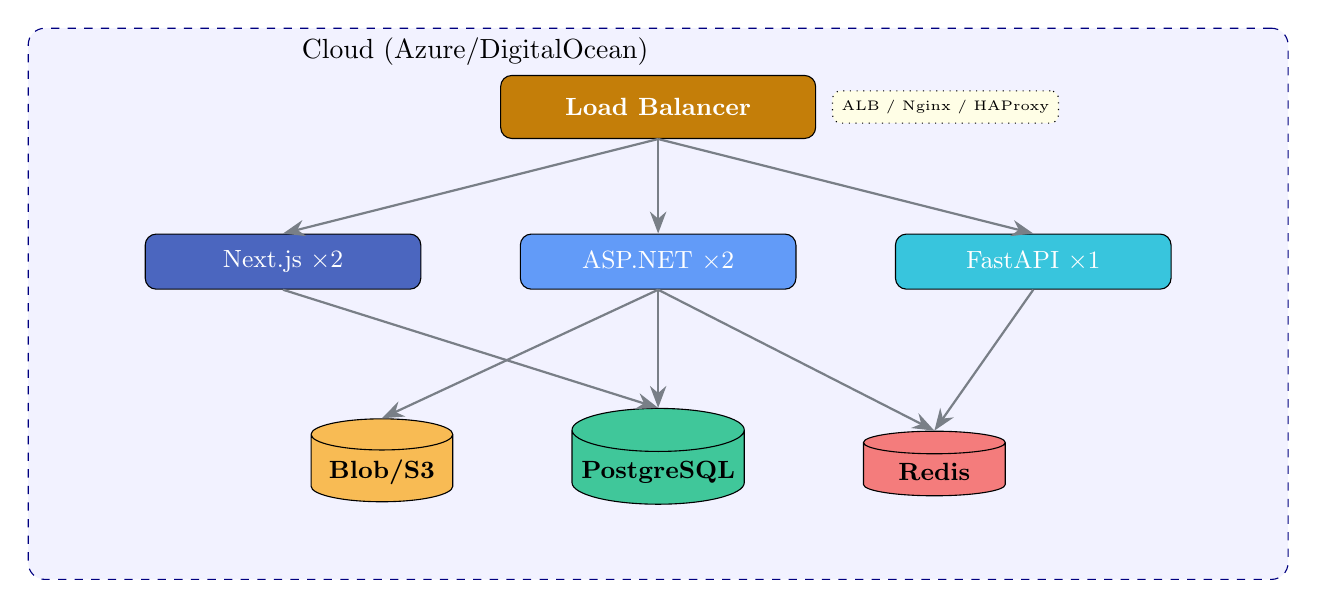
\begin{tikzpicture}[node distance=1cm]

% Cloud boundary
\node[container, fill=blue!5, draw=blue!50!black, minimum width=16cm, minimum height=7cm, label={[anchor=north east]Cloud (Azure/DigitalOcean)}] (cloud) {};

% Load balancer
\node[block, fill=warning!80!black, minimum width=4cm, minimum height=0.8cm] at (0,2.5) (lb) {Load Balancer};
\node[note, right=0.2cm of lb, font=\tiny] {ALB / Nginx / HAProxy};

% App services
\node[block, fill=primary!80, minimum width=3.5cm, minimum height=0.7cm, below left=1.2cm and 1cm of lb, font=\small] (fe) {Next.js $\times$2};
\node[block, fill=secondary!80, minimum width=3.5cm, minimum height=0.7cm, below=1.2cm of lb, font=\small] (be) {ASP.NET $\times$2};
\node[block, fill=accent!80, minimum width=3.5cm, minimum height=0.7cm, below right=1.2cm and 1cm of lb, font=\small] (ai) {FastAPI $\times$1};

\draw[arrow] (lb.south) -- (fe.north);
\draw[arrow] (lb.south) -- (be.north);
\draw[arrow] (lb.south) -- (ai.north);

% Data services
\node[db, fill=success!80, minimum width=2cm, minimum height=0.8cm, font=\small\bfseries, below=1.5cm of be] (pg) {PostgreSQL};
\node[db, fill=danger!70, minimum width=1.8cm, minimum height=0.7cm, font=\small\bfseries, right=1.5cm of pg] (rds) {Redis};
\node[db, fill=warning!70, minimum width=1.8cm, minimum height=0.7cm, font=\small\bfseries, left=1.5cm of pg] (s3) {Blob/S3};

\draw[arrow] (be.south) -- (pg.north);
\draw[arrow] (be.south) -- (rds.north);
\draw[arrow] (be.south) -- (s3.north);
\draw[arrow] (ai.south) -- (rds.north);
\draw[arrow] (fe.south) -- (pg.north);

\end{tikzpicture}
\caption{\textbf{Production Deployment Topology}}
\label{fig:deployment}
\end{figure}

\section{CI/CD Pipeline (GitHub Actions)}

\begin{figure}[H]
\centering

\begin{tikzpicture}[node distance=0.8cm]

\node[block, fill=dark!90, minimum width=3cm, minimum height=0.7cm, font=\small] (commit) {git push};

\node[block, fill=primary!80, minimum width=3cm, minimum height=0.7cm, right=1.5cm of commit, font=\small] (lint) {Lint + Type Check};

\node[block, fill=secondary!80, minimum width=3cm, minimum height=0.7cm, right=1.5cm of lint, font=\small] (test) {Run Tests (TDD Gate)};

\node[block, fill=accent!80, minimum width=3cm, minimum height=0.7cm, right=1.5cm of test, font=\small] (build) {Build Docker Images};

\node[block, fill=success!80, minimum width=3cm, minimum height=0.7cm, right=1.5cm of build, font=\small] (deploy) {Deploy to Staging};

\node[block, fill=danger!80, minimum width=3cm, minimum height=0.7cm, right=1.5cm of deploy, font=\small] (prod) {Production (Manual)}; 

\draw[arrow] (commit.east) -- (lint.west);
\draw[arrow] (lint.east) -- (test.west);
\draw[arrow] (test.east) -- (build.west);
\draw[arrow] (build.east) -- (deploy.west);
\draw[arrow] (deploy.east) -- (prod.west);

\end{tikzpicture}
\caption{\textbf{CI/CD Pipeline Stages}}
\label{fig:cicd}
\end{figure}

\section{Container Strategy (Docker)}

\begin{lstlisting}[style=code, language=bash, caption={docker-compose.yml (Development)}]
services:
  postgres:
    image: postgres:16-alpine
    volumes: [pgdata:/var/lib/postgresql/data]
    environment:
      POSTGRES_DB: tuitionhub
      POSTGRES_USER: tuitionhub
      POSTGRES_PASSWORD: ${DB_PASSWORD}
    ports: ["5432:5432"]

  redis:
    image: redis:7-alpine
    ports: ["6379:6379"]

  backend:
    build: ../backend
    depends_on: [postgres, redis]
    ports: ["5000:8080"]

  ai-service:
    build: ../ai-service
    depends_on: [redis]
    ports: ["8000:8000"]

  frontend:
    build: ../frontend
    depends_on: [backend]
    ports: ["3000:3000"]
\end{lstlisting}

\section{Estimated Resources (Initial Launch)}

\begin{longtable}{l|c|c|c|c}
\toprule
\textbf{Service} & \textbf{vCPU} & \textbf{RAM} & \textbf{Storage} & \textbf{Instances} \\
\midrule
\endhead
\bottomrule
\endfoot
Next.js Frontend  & 2 & 4 GB & --- & 2 \\
ASP.NET Core API  & 4 & 8 GB & --- & 2 \\
FastAPI AI Service & 2 & 4 GB & --- & 1 \\
PostgreSQL        & 4 & 16 GB & 100 GB SSD & 1 + 1 replica \\
Redis             & 2 & 4 GB & --- & 1 \\
\textbf{Monthly (est.)} & & & & \textbf{\$300--500} \\
\bottomrule
\end{longtable}

% ============================================================
\chapter{Development Roadmap}
% ============================================================

\section{Overview}

The roadmap is structured to solve the chicken-and-egg problem first, validate the business model early (payment integration in Phase 3), and progressively introduce monetization as marketplace liquidity grows.

\begin{figure}[H]
\centering

\begin{tikzpicture}[node distance=0.3cm]
\draw[thick, -{Stealth}] (0,0) -- (16,0);
\foreach \x/\l in {1/Setup,3/Profiles,5/Marketplace,7/Payments+Search,9/Comm,11/Admin,13/Monetize,15/Deliver}{
    \draw (\x*2-1,0.1) -- (\x*2-1,-0.1) node[below, font=\tiny] {\l};
}
\end{tikzpicture}
\caption{\textbf{8-Phase Build Timeline (16 Weeks)}}
\end{figure}

\section{Build Phases}

\begin{longtable}{p{0.7cm}|p{1.8cm}|p{2cm}|p{8cm}}
\toprule
\textbf{Ph} & \textbf{Weeks} & \textbf{Core Focus} & \textbf{Deliverables} \\
\midrule
\endhead
\bottomrule
\endfoot
1  & 1--2  & Foundation & \textbf{Git + GitHub setup.} Docker (PostgreSQL + Redis). Clean Architecture scaffolding + Auth (TDD). JWT + Refresh token rotation. Login/Register UI (mobile-first responsive). Service Worker + PWA manifest scaffolding. \\
2  & 3--4  & Profiles+Verif & User profiles. Tutor profile with academic/accreditation. Document upload. \textbf{Guardian verification}: phone OTP + optional NID. Admin verification flow. Profile UI with document preview. \\
3  & 5--6  & Marketplace+Pay & Tuition posts CRUD + Apply/Shortlist/Hire + Fuzzy search (English + Bangla). \textbf{bKash/Nagad payment integration}: commission calculation, transaction recording, payment gateway SDK. Job browsing UI. \\
4  & 7--8  & AI Matching & Rule-based matching engine (configurable weights from DB). pg\_trgm fuzzy search optimization. Salary prediction (LinearRegression). Fraud detection (rule-based + Isolation Forest). Trust score engine. Recommendation UI. \\
5  & 9--10 & Communication & SignalR chat (real-time, WebSocket with fallback). Multi-factor reviews (6 dimensions). Complaint workflow. Notification system (in-app + push via Service Worker). Chat UI + review form. \\
6  & 11--12 & Admin Panel & Super/Sub Admin dashboards. User management. Document verification queue. Financial reports. Audit log viewer. Admin panel UI with role-gated views. \\
7  & 13--14 & Monetization & \textbf{Tutor registration fee (BDT 500)} gate. \textbf{Premium Verified Badge (BDT 5,000)} with eligibility workflow. Featured posts. Ad placements. Revenue dashboard. Monetization UI + payment collection. \\
8  & 15--16 & Production & Security audit (OWASP Top 10). Load testing (k6). E2E tests (Playwright). Bangla search QA. PWA install test on Android/iOS. Staging deploy. Documentation. Production launch. \\
\bottomrule
\end{longtable}

\section{Go-to-Market Timeline}

\begin{longtable}{p{2cm}|p{3.5cm}|p{3cm}|p{4cm}}
\toprule
\textbf{Period} & \textbf{Product Stage} & \textbf{Business Stage} & \textbf{Key Metrics} \\
\midrule
\endhead
\bottomrule
\endfoot
Month 1--2 & MVP (Phases 1--2) & Supply acquisition & \textbf{2,000+ verified tutors in Dhaka} \\
Month 3--4 & Launch (Phases 3--4) & Demand activation & \textbf{500+ tuition posts, 50+ hires} \\
Month 5--6 & Growth (Phases 5--6) & Network effects & 30\% commission active, organic growth \\
Month 7--8 & Scale (Phases 7--8) & Monetization & BDT 500 fee, Premium Badge, expansion \\
Month 9--12 & Expansion & National rollout & Chattogram $\to$ Rajshahi $\to$ Khulna $\to$ Sylhet \\
\bottomrule
\end{longtable}

\section{TDD Workflow (Per Feature)}

\begin{enumerate}
    \item \textbf{Write a failing test} covering the acceptance criteria
    \item \textbf{Write the minimum code} to make the test pass
    \item \textbf{Refactor} while keeping tests green
    \item \textbf{Commit} with conventional commit message
    \item \textbf{Push to GitHub} --- CI runs test suite
\end{enumerate}

\begin{lstlisting}[style=code, language=bash, caption={Git Workflow Example}]
# Phase 1: Auth feature
git checkout -b feature/auth-register

# TDD cycle
dotnet test tests/TuitionHub.Api.Tests --filter "RegisterGuardian"  # Red
# ... implement RegisterCommandHandler ...
dotnet test tests/TuitionHub.Api.Tests --filter "RegisterGuardian"  # Green
# ... refactor ...

git add .
git commit -m "feat: add guardian registration with email OTP"
git push -u origin feature/auth-register
# → GitHub Actions runs full test suite
# → Create PR → merge to develop
\end{lstlisting}

% ============================================================
\chapter{Project Structure}
% ============================================================

\section{Complete Directory Layout}

\begin{lstlisting}[style=code, language=bash, caption={TuitionHub BD Full Project Tree}]
TuitionHub-BD/
├── frontend/                          # Next.js 15 Frontend
│   ├── app/
│   │   ├── (marketing)/               # Public landing pages
│   │   ├── (auth)/                    # Login, register, OTP
│   │   ├── (dashboard)/
│   │   │   ├── guardian/              # Guardian dashboard
│   │   │   ├── tutor/                 # Tutor dashboard
│   │   │   └── admin/                 # Admin panel
│   │   ├── api/                       # BFF API routes
│   │   ├── layout.tsx
│   │   └── page.tsx
│   ├── components/
│   │   ├── ui/                        # shadcn/ui primitives
│   │   ├── magicui/                   # Magic UI components
│   │   ├── forms/                     # Form components
│   │   └── layout/                    # Navbar, sidebar, footer
│   ├── lib/                           # Utilities, API client, Zod schemas
│   ├── hooks/                         # Custom React hooks
│   └── stores/                        # Zustand stores
│
├── backend/
│   ├── TuitionHub.Domain/             # Entities, Enums, Interfaces
│   ├── TuitionHub.Application/        # CQRS, MediatR handlers
│   ├── TuitionHub.Infrastructure/     # EF Core, Repositories, JWT, SignalR
│   └── TuitionHub.Api/               # Controllers, Middleware, Program.cs
│
├── ai-service/
│   ├── app/
│   │   ├── api/                       # FastAPI endpoints
│   │   ├── core/                      # Matching engine, scoring
│   │   ├── models/                    # Pydantic schemas
│   │   └── services/                  # Salary predictor, fraud detector
│   ├── tests/
│   └── Dockerfile
│
├── database/
│   ├── migrations/                    # EF Core migrations
│   ├── seeds/                         # Seed data
│   └── scripts/                       # Utility SQL scripts
│
├── docker/
│   ├── docker-compose.yml
│   └── Dockerfile.*
│
├── docs/                              # Design docs, API specs
├── .github/
│   └── workflows/                     # CI/CD pipelines
└── README.md
\end{lstlisting}

% ============================================================
\chapter{Appendix}
% ============================================================

\section{Conventional Commit Format}
\verb|type(scope): description|
\begin{itemize}
    \item \textbf{feat}: New feature
    \item \textbf{fix}: Bug fix
    \item \textbf{test}: Test additions or changes
    \item \textbf{refactor}: Code restructuring
    \item \textbf{chore}: Build, CI, config changes
    \item \textbf{docs}: Documentation
\end{itemize}

\section{Design Principles Applied}
\begin{itemize}
    \item \textbf{SOLID}: Single responsibility, Open-closed, Liskov substitution, Interface segregation, Dependency inversion
    \item \textbf{Clean Architecture}: Domain-centric, framework-agnostic core
    \item \textbf{CQRS}: Separated read/write models via MediatR
    \item \textbf{Repository Pattern}: Data access abstraction
    \item \textbf{Result Pattern}: Explicit success/failure, no exceptions for control flow
    \item \textbf{Outbox Pattern}: Reliable async event delivery
    \item \textbf{DRY}: Single source of truth for business rules
    \item \textbf{Pagination}: Cursor-based for large datasets
\end{itemize}

\section{Security Considerations}
\begin{itemize}
    \item HTTPS everywhere, HSTS headers
    \item JWT access tokens: 15 min expiry, in-memory storage
    \item Refresh tokens: 7 days, HTTP-only Secure cookies, rotation on use
    \item Password hashing: bcrypt (ASP.NET Identity default)
    \item Rate limiting: 100 req/min per user (Redis-backed)
    \item CORS: Whitelisted origins only
    \item SQL injection: prevented by EF Core parameterized queries
    \item XSS: React's JSX sanitization + Content Security Policy
    \item CSRF: Anti-forgery tokens on state-changing endpoints
    \item File upload: Size limits, MIME validation, virus scanning
    \item Secrets: Environment variables / Azure Key Vault
\end{itemize}

\section{Monitoring \& Observability}
\begin{itemize}
    \item \textbf{Logging}: Serilog (structured) + Grafana Loki
    \item \textbf{Metrics}: Prometheus --- request rate, latency, error rate, DB query perf
    \item \textbf{Tracing}: OpenTelemetry distributed traces across .NET $\to$ FastAPI $\to$ PostgreSQL
    \item \textbf{Errors}: Sentry for exception aggregation
    \item \textbf{Uptime}: Health check endpoints (./well-known/health)
    \item \textbf{Alerts}: PagerDuty / Slack webhooks on critical failures
\end{itemize}

\end{document}
